\documentclass[prd,preprintnumbers,twocolumn,eqsecnum,floatfix,a4paper,nofootinbib,superscriptaddress]{revtex4}
\usepackage{color}
\usepackage{calc}
\usepackage{amsmath,amssymb,graphicx}
\usepackage{amssymb,amsmath}
\usepackage{bm}
\usepackage{microtype}
\usepackage{booktabs}
\usepackage{times}
\usepackage{subfigure}
\usepackage[varg]{txfonts}
\usepackage[colorlinks, pdfborder={0 0 0}]{hyperref}
\usepackage[utf8]{inputenc}
\definecolor{LinkColor}{rgb}{0.75, 0, 0}
\definecolor{CiteColor}{rgb}{0, 0.5, 0.5}
\definecolor{UrlColor}{rgb}{0, 0, 0.75}
\hypersetup{linkcolor=LinkColor}
\hypersetup{citecolor=CiteColor}
\hypersetup{urlcolor=UrlColor}
\maxdeadcycles=1000
\allowdisplaybreaks
\textwidth 7 in
\hoffset -0.1in
\textheight 10in
\DeclareFontFamily{OT1}{pzc}{}
\DeclareFontShape{OT1}{pzc}{m}{it}{<-> s * [1.10] pzcmi7t}{}
\DeclareMathAlphabet{\mathpzc}{OT1}{pzc}{m}{it}
\newcommand{\comment}[1]{\textcolor{blue}{\textit{#1}}}
\newcommand{\ajith}[1]{\textcolor{red}{\textit{Ajith:#1}}}
\newcommand{\checkthis}{\textcolor{magenta}{(CHECKTHIS)}}
\newcommand{\vijay}[1]{\textcolor{cyan}{Vijay: #1}}
\newcommand{\io}{\iota}
\newcommand{\p}{\phi}
\newcommand{\vp}{\varphi}

\newcommand{\h}{\mathpzc{h}}
\newcommand{\Hhat}{\hat{\mathpzc{H}}}
\newcommand{\B}{\mathpzc{B}}
\newcommand{\hlm}{\mathpzc{h}_{\ell m}}
\newcommand{\xilm}{\xi_{\ell m}}
\newcommand{\Ylm}{{Y}^{-2}_{\ell m}}
\newcommand{\Y}{{Y}^{-2}}
\newcommand{\hc}{h_\times}
\newcommand{\hp}{h_+}
\newcommand{\Fc}{F_\times}
\newcommand{\Fp}{F_+}
\newcommand{\Mf}{M_f}
\newcommand{\cA}{\mathpzc{A}}
\newcommand{\lm}{_{\ell m}}
\newcommand{\deff}{d_\mathrm{eff}}
\newcommand{\rmi}{\mathrm{i}}
\newcommand{\blambda}{\bm{\lambda}}
\newcommand{\btheta}{\bm{\theta}}
\newcommand{\Mo}{M_{\odot}}
\newcommand{\FFe}{\mathrm{FF}_\mathrm{eff}}
\newcommand{\FF}{\mathrm{FF}}
\newcommand{\e}{\mathrm{e}}
\newcommand{\rhoopt}{\rho_\mathrm{opt}}
\newcommand{\rhosubopt}{\rho_\mathrm{subopt}}
\newcommand{\fqnm}{f}
\newcommand{\sigmaqnm}{\sigma}
\newcommand{\n}{\mathbf{n}}
\newcommand{\bxi}{\bm{\xi}}
\newcommand*{\skymapscale}{0.5}
\newcommand*{\paramestscale}{0.455}

\begin{document}

\newcommand{\be}{\begin{equation}}
\newcommand{\ee}{\end{equation}}
\newcommand{\ber}{\begin{eqnarray}}
\newcommand{\eer}{\end{eqnarray}}
\def\bea{\begin{eqnarray}}
\def\eea{\end{eqnarray}}
\newcommand{\etal}{\emph{et al}}

\title{Accurate inspiral-merger-ringdown gravitational waveforms \\ for non-spinning black-hole binaries including the effect of subdominant modes}
% \author{Ajit Kumar Mehta}
% \affiliation{International Centre for Theoretical Sciences, Tata Institute of Fundamental Research, Bangalore 560012, India}
% \author{Chandra Kant Mishra}
% \affiliation{International Centre for Theoretical Sciences, Tata Institute of Fundamental Research, Bangalore 560012, India}
% \affiliation{Indian Institute of Technology, Madras, Chennai 600036, India}
% \author{Vijay Varma}
% \affiliation{Theoretical Astrophysics, 350-17, California Institute of Technology, Pasadena, CA 91125, USA}
% \affiliation{International Centre for Theoretical Sciences, Tata Institute of Fundamental Research, Bangalore 560012, India}
% \author{Parameswaran~Ajith}
% \affiliation{International Centre for Theoretical Sciences, Tata Institute of Fundamental Research, Bangalore 560012, India}
% \affiliation{Canadian Institute for Advanced Research, CIFAR Azrieli Global Scholar, MaRS Centre, West Tower, 661 University Ave., Suite 505, Toronto, ON M5G 1M1, Canada}

\begin{abstract}
\end{abstract}
\preprint{LIGO-P1700160-v3}
\maketitle
%%%%%%%%%%%%%%%%%%%%%%%%%%%%%%%%%%%%%%%%%%%%%%%%%%%%%%%%%%%%%%%%%%%%%%%%%%%%%%%%%%%%%%%%%%%%%%%%%%%%%%%%%%%%%%%%%%%%%%%%%%%%%%%%%%%%%%%%%%%%%%%`
\section{Introduction}
%%%%%%%%%%%%%%%%%%%%%%%%%%%%%%%%%%%%%%%%%%%%%%%%%%%%%%%%%%%%%%%%%%%%%%%%%%%%%%%%%%%%%%%%%%%%%%%%%%%%%%%%%%%%%%%%%%%%%%%%%%%%%%%%%%%%%%%%%%%%%%%`
\section{Data analysis method}
\subsection{Waveform model}
Gravitational wave radiation emitted by a binary black hole in GR can be written as a linear combination of the `plus' and `cross' polarisations : $\h(t) := h_+(t) - i \, h_\times(t)$, which can be expanded in a basis of spin $-2$ weighted spherical harmonics~\cite{NewmanPenrose} as:
\begin{equation}
\h(t; \n, \blambda, \Delta \blambda)= \frac{1}{d_L} \sum _{\ell=2}^{\infty} \sum _{m=-\ell}^{\ell} {\Ylm} (\n) \, {{\hlm}(t; {\blambda})}, 
\label{eq:spherical_harmonics}
\end{equation}
where ${\Ylm}$ are the basis functions of spin $-2$ spherical harmonics, $\n := \{\iota, \varphi_0\}$ define the direction of radiation in the source frame, $d_L$ is  the luminosity distance to the binary, and ${\h}_{lm}(t; \blambda)$ are the spherical harmonic modes of the waveform. The inclination angle $\iota$ is measured with respect to the orbital angular momentum of the binary. 

The spherical harmonic modes, ${\h}_{lm}(t; \blambda)$, are purely functions of the intrinsic parameters $\blambda$ of the system, while all the angular dependence is captured by the spherical harmonic basis functions ${\Ylm}$.  Here, we consider the black holes to be non-spinning and the binary to be quasi-circular. Hence $\blambda$ consists of only the component masses $m_1$ and $m_2$ of the black holes. However, it is more convenient to use a reparameterization of the mass plane into the \emph{chirp mass} $M_c := {(m_1m_2)^{3/5}}/{(m_1+m_2)^{1/5}}$ and asymmetric mass ratio $q = m_2/m_1 \leq 1$. In GR, the leading contribution in gravitational radiation comes from the quadrupole modes ($\ell = 2, m = \pm 2$). The relative contribution of the higher modes depends on the mass ratio $q$ and the inclination angle $\iota$.  Non-quadrupole modes becomes important when the black holes have significantly unequal masses and larger inclination angle. This multipolar structure (i.e., spherical harmonic modes) of the waveform ${\h}_{lm}(t)$ is completely determined by the set of intrinsic parameters $\blambda := \{M_c, q\}$.

\subsection{Signal model}
The gravitational wave strain observed by a detector can be expressed as
\begin{equation}
h(t) = F_+(\theta, \phi, \psi) \, h_+(t-t_0) + F_{\times}(\theta, \phi, \psi)\, {h}_{\times}(t-t_0), 
\label{eq:det_response}
\end{equation}
where $F_+$ and $F_\times$ are the antenna pattern functions of the GW detector, $t_0$ is the time of arrival of the signal at the detector, and $(\theta, \phi), \psi$ define the source location and polarisation angle of the gravitational wave, respectively. For coalescing BBH systems in quasi-circular orbits, the measured strain $h(t)$ is therefore described by a set of \emph{intrinsic} parameters $\blambda = \{M_c, q\}$ and \emph{extrinsic} parameters  $\btheta := \{t_0, \iota, \varphi_0, d_L, \theta, \phi, \psi\}$ in GR. In addition to the parameters that describe signals in GR, we introduce a set of intrinsic parameters $\Delta \blambda$ and extrinsic parameters $\Delta \btheta$  which captures any possible departure from GR (details in Section \ref{sec3} and Section \ref{sec4}). The deviation parameters $\Delta \blambda$ ($\Delta \btheta$) describes difference between the intrinsic (extrinsic) parameters used to generate the dominant and subdominant modes or the `plus' and `cross' polarizations.  The combined set of parameters is denoted as $\bxi = \{\blambda, \btheta, \Delta \blambda, \Delta \btheta\}$. 

\subsection{Bayesian analysis}
We assume that the data $d(t) = n(t) + h(t)$ from the gravitational wave detector contains both the observed signal $h(t)$ given in Eq.~(\ref{eq:det_response}) and a  stationary Gaussian noise component $n(t)$. Given data $d(t)$, we compute the probability distribution of the combined set of parameters ${\bxi}$ of a paricular hypothesis $H$ associated with a waveform model (details in Section \ref{sec3} and Section \ref{sec4}) using the Bayes theorem: 
\begin{equation}
P({\bxi} \, | \, d, H) = \frac{P({\bxi} \, | \, H) \, P (d \, | \, {\bxi}, H)}{P(d \, | \, H)}.
\label{eq:Bayes_theorem}
\end{equation} 
The \emph{posterior} probability density $P({\bxi}\,|\,d,H)$ that the data contains a signal with parameters $\bxi$ is determined by the \emph{prior} probability distribution $P({\bxi} \, | \, H)$ and the \emph{likelihood} $P (d \, | \, {\bxi}, H)$. Prior $P({\bxi} \, | \, H)$ denotes the probability of the parameters given by the Hypothesis (or signal model). In this paper, the prior density function on the location of the source is  taken  to  be  isotropically  distributed  on  the  sphere of  the  sky,  with
$P({dL} \, | \, H)=d_{L}^{2}$. Furthermore, we use an  isotropic  prior  on  the  orientation  of  the  binary: $P({\iota,\varphi_0,\psi} \, | \, H)=sin\iota$. For all other parameters in $\bxi$, we use uniform prior distribution. The likelihood $P (d \, | \, {\bxi}, H)$ gives the probability of observing data $d(t)$ given the model parameter $\bxi$; and $P(d \, | \, H)$ is a normalization constant, called the \emph{evidence} or the \emph{marginal likelihood}, expressed as:
 \begin{equation}
 P(d \, | \, H)=\int p(d|\bxi)p(\bxi)d\bxi.
 \label{eq:evidence}
 \end{equation}
For stationary Gaussian noise with power spectral density $S_n(f)$, the likelihood is written as:
\begin{equation}
P (d \, | \, {\bxi}, H) = \text{exp}\left[ -\frac{1}{2}\int_{f_\mathrm{low}}^{f_\mathrm{high}} \frac{|\tilde{d}(f) - \tilde{h}(f;{\bxi}, H)|^2}{S_n(f)}df\right],
\end{equation}
where $\tilde{d}(f)$ and $\tilde{h}(f)$ are the Fourier transforms of $d(t)$ and $h(t)$, respectively. The limits of the integration $f_\mathrm{low}$ and $f_\mathrm{high}$ define the sensitivity bandwidth of the detector. In this work, we use a network of three LIGO-VIRGO detectors. We assume that the noise is uncorrelated in each detector. The network likelihood for data obtained from three detectors can thus be written as the product of the likelihoods in each detector
\begin{equation}
P (d \, | \, {\bxi}, H, S_n(f)) = \prod_{i \epsilon {H,L,V}} P (d_{i} \, | \, {\bxi}, H, S_{n_{i}}(f)).
\end{equation}

Using the Bayesian framework described above, we estimate $\bxi$ by stochastically sampling over the entire parameter space of interest. We use python-based affine-invariant ensemble sampler \texttt{emcee}~\cite{foreman2013emcee} for Markov chain Monte Carlo (MCMC) proposed by \cite{goodman2010ensemble} to obtain the posterior distribution $P(\bxi \, | \, d, H)$ of the full parameter set. Posterior distributions of particular parameters of interest, for example,  the set of parameters ${\Delta \blambda, \Delta \btheta}$, describing deviation from the GR prediction of a BBH signal, are computed  by marginalizing the posterior over all other parameters $\{\blambda, \btheta\}$. If the data is consistent with a BBH signal in GR, we expect $P(\Delta \blambda \, | \, d, H)$ to be consistent with zero. 

\subsection{Constraining deviation parameters  using GR waveforms}
We employ the recent phenomenological inspiral-merger-ringdown waveform model proposed by~\cite{Mehta:2017jpq}, which provide accurate Fourier-domain models of three sub-dominant spherical harmonic modes ($(\ell = 2, m=\pm1)$, $(\ell = 3, m=\pm3)$, $(\ell = 4, m = \pm4)$) apart from the dominant $(\ell = 2, m = \pm2)$ mode of the expected GW signals from non-spinning BBHs. The other spherical harmonic modes neglected in this work only introduce an inaccuracy (mismatch) of less than 1\% in the waveforms~\cite{Mehta:2017jpq}. We combine these signals with stationary Gaussian noise with power spectral density anticipated in Advanced LIGO's ``high-power, zero-detuning'' configuration~\cite{aLIGOZeroDetHighPower}, making use of Eqs.~(\ref{eq:spherical_harmonics}) and (\ref{eq:det_response}), and simulate GR observations. We consider binaries with total mass $M := m_1 + m_2$ in the range $40 M_\odot$ -- 200 $M_\odot$ with mass ratio $q := m_2/m_1$ in the range 1/9 -- 1, with varying inclination angles $\iota=\{30^{\circ},45^{\circ},60^{\circ},80^{\circ},90^{\circ}\}$. Using these simulated GR events, we compute the marginalized posterior distribution of the deviation parameters  $\{\Delta \blambda, \Delta \btheta\}$. In order to compute the constraints on these parameters, we calculate the 90\% probability interval. Parameters which are recovered with greatest precision from the simulated GR signal will result smaller values for the credible interval and therefore would give more stringent test of GR with actual observation.

%%%%%%%%%%%%%%%%%%%%%%%%%%%%%%%%%%%%%%%%%%%%%%%%%%%%%%%%%%%%%%%%%%%%%%%%%%%%%%%%%%%%%%%%%%%%%%%%%%%%%%%%%%%%%%%%%%%%%%%%%%%%%%%%%%%%%%%%%%%%%%%`
\section{Consistency between spherical harmonic modes}
\label{sec3}
In this section, we present two tests of GR based on checking the consistency between different spherical harmonic modes of the observed signal. Our strategy, developed below, is to introduce extra parameters in the higher order modes of radiation, both intrinsic and extrinsic, that describe inconsistency between different modes and to constrain them using a Bayesian framework. 

\subsection{Consistency between parameters estimated from different modes}
\label{sec3a}
The first test we consider broadly follows the outline presented in ~\cite{dhanpal2018} to check for the consistency of intrinsic parameters $\blambda := \{M_c, q\}$ estimated from the dominant mode and the higher order modes. According to this, we would estimate the chirp mass and asymmetric mas ratio of the BBH from the leading quadrapolar mode of the observed signal. Independently, we would obtain the same estimates from the higher order modes. In GR, these two estimates of $M_c$ and $q$ should match. 

The test is formulated in the following way: we rewrite Eq.~(\ref{eq:spherical_harmonics}) by splitting the contributions from the dominant $(\ell = 2, m = \pm 2)$ mode of gravitational radiation, and the sub-dominant (higher order) modes 
\begin{eqnarray}
\h(t; \n, \blambda, \Delta \blambda) & = & \sum_{m = \pm2} Y^{-2}_{2m} (\n) {\h}_{2m}(t, \blambda)  \nonumber \\ 
& + & \sum _{\text{H.O.M}} \Ylm (\n) \hlm(t, \blambda+\Delta \blambda)
\label{eq:test_HM}
\end{eqnarray}
where the sum in the second term on the RHS is just over the higher-order modes and incorporate a deviation $\Delta \blambda := \{\Delta M_c, \Delta q\}$ in the set of intrinsic parameters that describe the higher order modes. In the absence of any departure from GR, we expect $\Delta \blambda $ to be consistent with zero. While ~\cite{dhanpal2018} focuses on one performing this test with only one arbitrary detector, we generalize the test in realistic three detector LIGO-VIRGO setup.

%%%%%%%%%%%%%%%%%%%%%%%%%%%%%%%%%%%%%%%%%%%%%%%%%%%%%%%%%%%%%%%%%%%%%%%%%%%%%%%%%%%%%%%%%%
\begin{figure}[htb] \begin{center}
		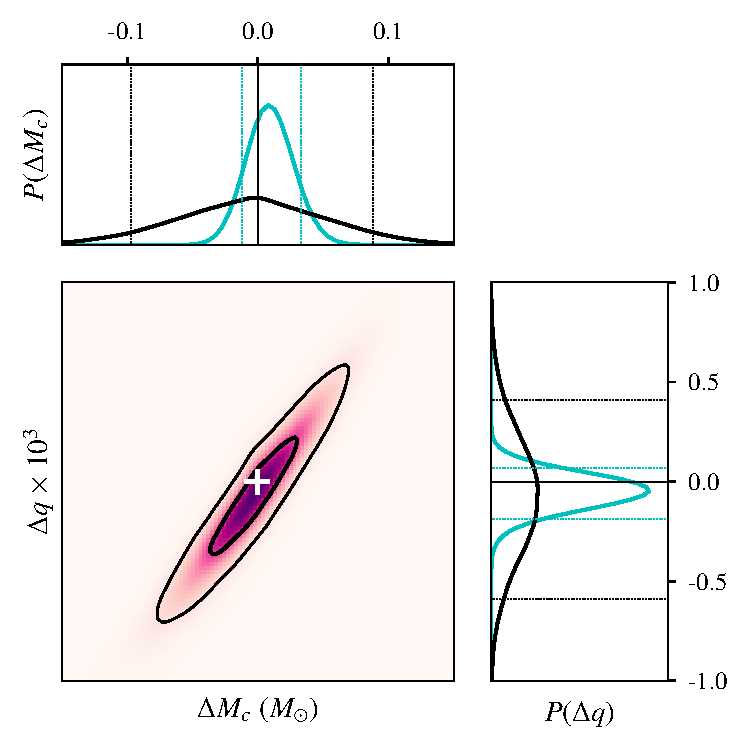
\includegraphics[width=3.4in]{figs/hm_mcq_GR.pdf}
		\caption{(\textbf{Middle panel}): the thick (thin) contours show the 50\% (90\%) credible regions in the joint posteriors of two parameters $\Delta M_c$ and $\Delta q$ that describe deviations in the estimated parameters using the quadrupole and non-quadrupole modes, estimated from a simulated GR signal. (\textbf{Side panels}): Black histograms show the 2-dimensional marginalized posteriors in $\Delta M_c$ and $\Delta q$, while the cyan histograms show the 1-dimensional posteriors in $\Delta M_c$ and $\Delta q$ estimated from the data by introducing only one deviation parameter (say, $\Delta M_c$) at a time, keeping the other fixed (say, $\Delta q = 0$). The posteriors are fully consistent with the GR prediction of $\Delta M_c = \Delta q = 0$ (shown by a ``+'' sign in the center panel and by thin black lines in side panels). The dotted lines mark the 90\% credible regions. The simulated GR signal corresponds to a binary with total mass $M = {80}M_\odot$ and mass ratio $q = 1/9$ and an inclination angle $\iota = {60^\circ}$ observed by Advanced LIGO-VIRGO detectors network with an optimal SNR of 25. }
		\label{fig:posterior_BBH_GR_inj}
\end{center} \end{figure}
%%%%%%%%%%%%%%%%%%%%%%%%%%%%%%%%%%%%%%%%%%%%%%%%%%%%%%%%%%%%%%%%%%%%%%%%%%%%%%%%%%%%%%%%%%

We consider two different ways to perform the test. First, we introduce \emph{one} deviation parameter at a time. That is, $\Delta\blambda = {\Delta M_c}$ or $\Delta\blambda = {\Delta q}$. We then consider introducing a concurrent deviation in \emph{two} parameters $\Delta \blambda = \{\Delta M_c, \Delta q\}$. In Fig. 
~\ref{fig:posterior_BBH_GR_inj}, we show the results of the tests performed with GR waveform by varying either one parameter or two parameters, for a binary with total mass $M = 80M_{\odot}$, mass ratio $q=1/9$, inclination angle $ {\iota}=60^{\circ} $ producing a signal-to-noise ratio  (SNR)  of 25 (SNR in higher modes is $\sim 10$). The posterior probability density for both the parameters $\Delta q$ and $\Delta M_c$ are consistent with zero as one expect in GR. Furthermore, the deviation parameters are found to be better constrained when only one deviation parameter is allowed to vary at a time (either $\Delta M_c$ or $\Delta q$). This suggests that a consistency test with only one deviation parameter in the higher modes would allow a more efficient test. In the subsequent analysis, we therefore focus on varying only one deviation parameter at a time. 

Up next, in Fig. \ref{fig:hm_mcq_compare-1det_3det_GR_inj} we show that, as expected, the width of the posteriors of the deviation parameters become smaller when we perform the test with a network of three Advanced LIGO-VIRGO detectors instead of using only one Advanced LIGO detector. 

 

%%%%%%%%%%%%%%%%%%%%%%%%%%%%%%%%%%%%%%%%%%%%%%%%%%%%%%%%%%%%%%%%%%%%%%%%%%%%%%%%%%%%%%%%%%
\begin{figure}[htb] \begin{center}
		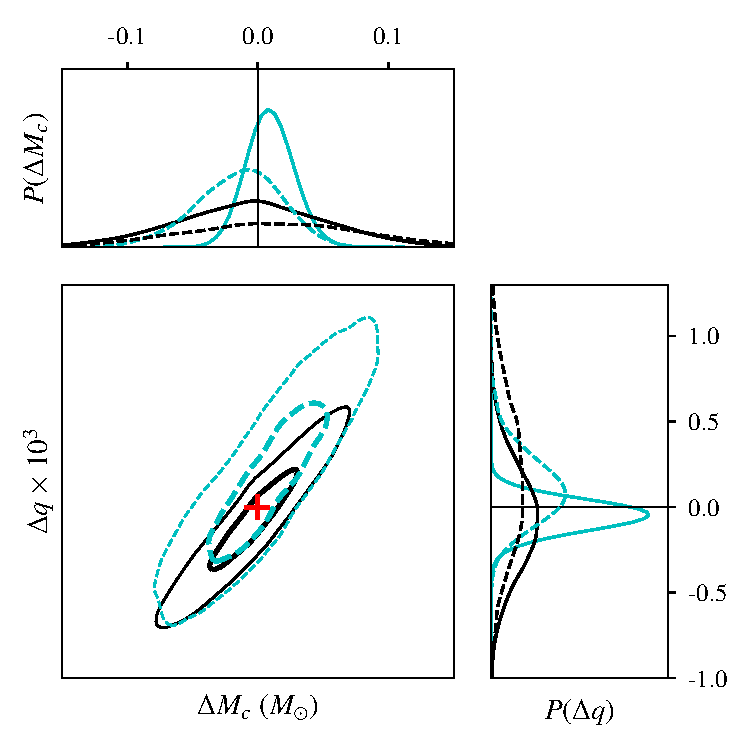
\includegraphics[width=3.4in]{figs/hm_mcq_1det_3det_compare_GR.pdf}
		\caption{(\textbf{Middle panel}): the thick (thin) contours show the 50\% (90\%) credible regions in the joint posteriors of two parameters $\Delta M_c$ and $\Delta q$ that describe deviations in the estimated parameters using the quadrupole and non-quadrupole modes, estimated from a simulated GR signal. Solid black lines indicates the joint posterior obtained by network of three detectors in Advanced LIGO-VIRGO setup, while dashed cyan lines show the  joint posterior obtained with only one Advanced LIGO detector. (\textbf{Side panels}): Black histograms show the 2-dimensional marginalized posteriors in $\Delta M_c$ and $\Delta q$, while the cyan histograms show the 1-dimensional posteriors in $\Delta M_c$ and $\Delta q$ estimated from the data by introducing only one deviation parameter (say, $\Delta M_c$) at a time, keeping the other fixed (say, $\Delta q = 0$). The posteriors are fully consistent with the GR prediction of $\Delta M_c = \Delta q = 0$ (shown by a ``+'' sign in the center panel and by thin black lines in side panels).  Solid lines indicates the posterior recovered by network of three detectors in Advanced LIGO-VIRGO setup and dashed lines implies the posterior obtained with only one Advanced LIGO detector. The simulated GR signal corresponds to a binary with total mass $M = {80}M_\odot$ and mass ratio $q = 1/9$ and an inclination angle $\iota = {60^\circ}$ observed either by one Advanced LIGO detector or network of LIGO-VIRGO detectors with an optimal SNR of 25. }
		\label{fig:hm_mcq_compare-1det_3det_GR_inj}
	\end{center} \end{figure}
	%%%%%%%%%%%%%%%%%%%%%%%%%%%%%%%%%%%%%%%%%%%%%%%%%%%%%%%%%%%%%%%%%%%%%%%%%%%%%%%%%%%%%%%%%%
 Figures~\ref{fig:delmc_delq_varyingM} and \ref{fig:delmc_delq_varyingq} show the 90\% credible intervals of the posteriors of the deviation parameters for binaries with varying masses, mass ratios and inclination angles. In all cases, we set the SNR to be {25}.  We find that binaries with large mass ratios ($q < 1/ 2$) and inclination angles ($\iota > 60 ^\circ $) will allow precision tests of the GR predictions, reaching statistical uncertainties of $< 10^{-3}$ for $\Delta q$ and $< 10^{-2}$ for the dimensionless deviation parameter $\Delta M_c/M_c$. We note that the 90\% interval for both the deviation parameters decreases slightly compared to the earlier reported values in~\cite{dhanpal2018}.
 
 \begin{figure}[tbh]
 	\begin{center}
 		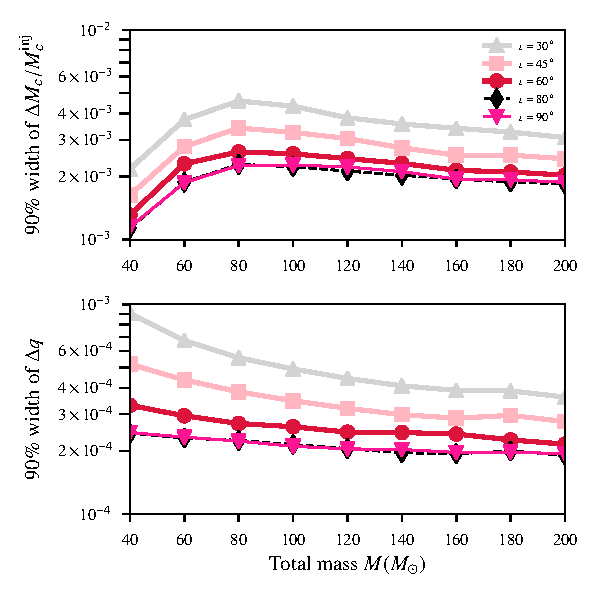
\includegraphics[scale=0.8]{figs/hm_9dim_dmcbymcinj_dq_diff_M.pdf}
 	\end{center} 
 	\caption{The figure shows the width of the 90$\%$ confidence limit of the deviation parameters $\Delta M_c$ and $\Delta q$ for binaries with different total mass (horizontal axis) and inclination angles $\iota$ (legends). All binaries have an asymmetric mass ratio $q=1/9$.}
 	\label{fig:delmc_delq_varyingM}
 \end{figure}
 
 \begin{figure}[tbh]
 	\begin{center}
 		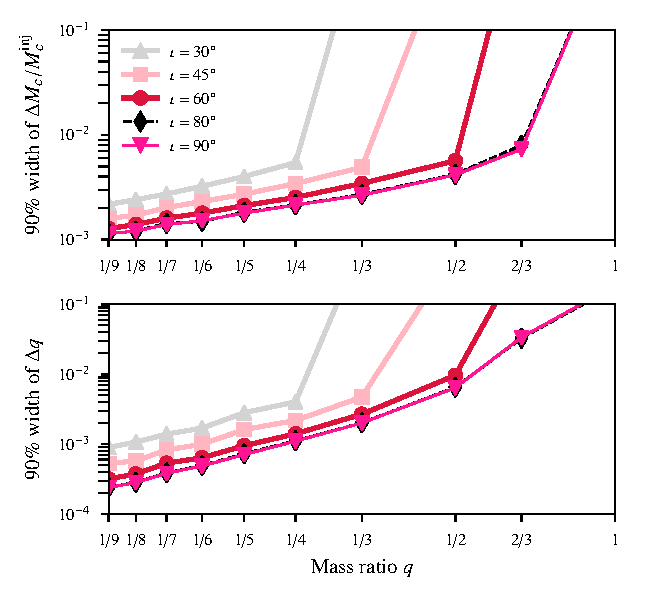
\includegraphics[scale=0.8]{figs/hm_9dim_dmcbymcinj_dq_diff_q.pdf}
 	\end{center} 
 	\caption{Same as Fig.~\ref{fig:delmc_delq_varyingM}, except that the horizontal axis reports the mass ratio $q$. All binaries correspond to a total mass $40M_{\odot}$.}
 	\label{fig:delmc_delq_varyingq}
 \end{figure}
%%%%%%%%%%%%%%%%%%%%%%%%%%%%%%%%%%%%%%%%%%%%%%%%%%%%%%%%%%%%%%%%%%%%%%%%%%%%%%%%%%%%%%%%%%%%%%%%%%%%%%%%%%%%%%%%%%%%%%%%%%%%%%%%%%%%%%%%%%%%%%%`
\subsection{Consistency between the amplitude and phase from different modes}
While one can estimate the intrinsic parameters (chirp mass and mass ratio of the BBH) from the quadrapolar mode and the higher order modes independently and formulate an efficient test of GR, that is not the only way to do so. Another interesting parameterized test of GR with using multipolar structure of the waveform would involve introducing generic possible deviation parameters in the amplitudes of the higher order modes. We consider three different  ways to formulate such tests:

 \begin{enumerate}
 	\item We split the contributions from the dominant $(\ell = 2, m = \pm 2)$ mode of gravitational radiation, and the higher order modes in Eq.~(\ref{eq:spherical_harmonics}) and introduce a generic extrinsic deviation parameter $\Delta \btheta=\{c_1\}$ common for all the higher modes considered i.e. $(\ell = 2, m=\pm1)$, $(\ell = 3, m=\pm3)$, $(\ell = 4, m = \pm4)$.
 	\begin{eqnarray}
 	{\h}(t; n, \blambda, \Delta \blambda) & = & \frac{1}{d_L} \sum_{m = \pm2} Y^{-2}_{2m} (n) {\h}_{2m}(t, \blambda)  \nonumber \\ 
 	& + & \frac{(1+{c_1})}{d_L} \sum _{\text{H.O.M}} \Ylm (n) \hlm(t, \blambda),
 	\label{eq:test_c1}
 	\end{eqnarray}
 	where  H.O.M represents the higher order modes, and $\blambda$ be the intrinsic parameters. 	
 
 %%%%%%%%%%%%%%%%%%%%%%%%%%%%%%%%%%%%%%%%%%%%%%%%%%%%
 \begin{figure}[tbh]
 	\begin{center}
 		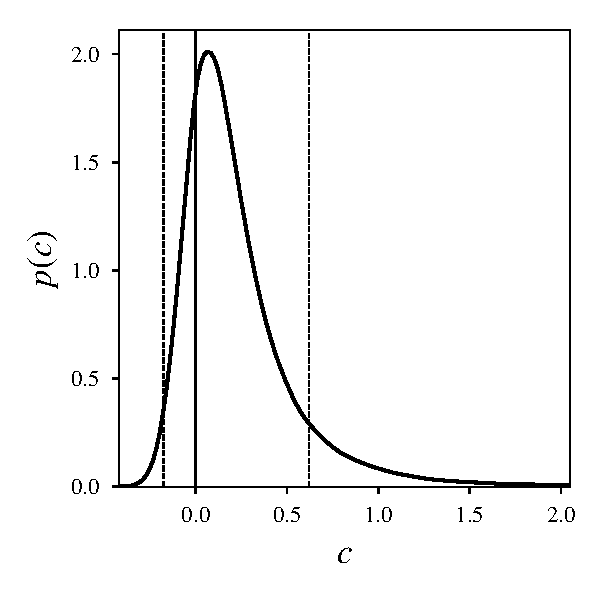
\includegraphics[scale=0.5]{figs/hist_c1_M_80_q_9_snr_25.pdf}
 	\end{center} 
 	\caption{\textbf{FILLER} : The figure shows the posterior probability distribution of the deviation parameter $c_1$ estimated from the same simulated GR observation in \ref{fig:posterior_BBH_GR_inj}. Thin black lines shows the expected value in GR. The dotted lines mark the 90\% credible regions. }
 	\label{fig:c1_hist}
 \end{figure}
 %%%%%%%%%%%%%%%%%%%%%%%%%%%%%%%%%%%%%%%%%%%%%%%%%%%%%
 
 	\item We then generalize the test by introducing a set of two different deviation parameter $\Delta \btheta=\{c_2, c_{34}\}$, where $c_2$ indicates the possible modification in the  $(\ell = 2, m=\pm1)$ mode and $c_{34}$ encodes a common deviation in $(\ell = 3, m=\pm3)$ and $(\ell = 4, m = \pm4)$ modes.
 	\begin{eqnarray}
 	{\h}(t; n, \blambda, \Delta \blambda) & = & \frac{1}{d_L} \sum_{m = \pm2} Y^{-2}_{2m} (n) {\h}_{2m}(t, \blambda)  \nonumber \\ 
 	& + & \frac{(1+{c_2})}{d_L} \sum_{m = \pm1} Y^{-2}_{2m} (n) {\h}_{2m}(t, \blambda) \nonumber\\
 	& + & \frac{(1+{c_{34}})}{d_L} \sum _{\text{33,44}} \Ylm (n) \hlm(t, \blambda),
 	\label{eq:test_c2_c34}
 	\end{eqnarray}

	
 	\item In a futher generalization, we keep the amplitude of the quadrapole mode as well as the $(\ell = 2, m=\pm1)$ mode as predicted in GR and choose a set of two different deviation parameter $\Delta \btheta=\{c_3, c_{4}\}$ in the amplitudes of  $(\ell = 3, m=\pm3)$ mode and $(\ell = 4, m = \pm4)$ mode respectively.
 	\begin{eqnarray}
 	{\h}(t; n, \blambda, \Delta \blambda) & = & \frac{1}{d_L} \sum_{m = \pm2,\pm1} Y^{-2}_{2m} (n) {\h}_{2m}(t, \blambda)  \nonumber \\ 
 	& + & \frac{(1+{c_3})}{d_L} \sum_{m = \pm3} Y^{-2}_{3m} (n) {\h}_{3m}(t, \blambda) \nonumber\\
 	& + & \frac{(1+{c_{4}})}{d_L} \sum _{m=\pm4} Y^{-2}_{4m} (n) {\h}_{4m}(t, \blambda),
 	\label{eq:test_c3_c4}
 	\end{eqnarray}
 \end{enumerate}

The set of deviation parameters $\Delta \btheta=\{c_1\}$, $\Delta \btheta=\{c_3, c_{4}\}$ and $\Delta \btheta=\{c_3, c_{4}\}$ encodes possible departure from  GR. If there is no evidence of GR to be violated, all these deviation parameters would be consistent with zero. On the other hand, if GR is wrong, the posterior of these parameters $\Delta \btheta$, estimated from observations, would show a discrepancy with the expected value i.e. $\Delta \btheta=0$. In Fig. \ref{fig:c1_hist}, we show an example of posterior distribution of $c_1$ from a simulated GR event with SNR 25, for a binary with total mass $M = 80M_{\odot}$, mass ratio $q=1/9$ and inclination angle $ {\iota}=60^{\circ} $.  We see that the posterior distribution are consistent with zero. Figure \ref{fig:constraint_c1} shows the 90\% credible interval for $c_1$.  The posterior probability densities of $\Delta \btheta=\{c_2, c_{34}\}$ and $\Delta \btheta=\{c_3, c_{4}\}$ estimated from the same simulated GR event (shown in Fig. \ref{fig:c2_c34} and \ref{fig:c3_c4}) are also found to be consistent with zero. We now estimate the expected constraints on these deviation parameters by injecting simulated GR waveforms. The constraints on $\btheta=\{c_3, c_{4}\}$ and $\Delta \btheta=\{c_3, c_{4}\}$ calculated from GR events are presented in Fig. \ref{fig:bounds_c2}, Fig. \ref{fig:bounds_c34}, Fig. \ref{fig:bounds_c3} and Fig. \ref{fig:bounds_c4}.


%%%%%%%%%%%%%%%%%%%%%%%%%%%%%%%%%%%%%%%%%%%%%%%%%%%%%
\begin{figure}[h]
	\begin{center}
		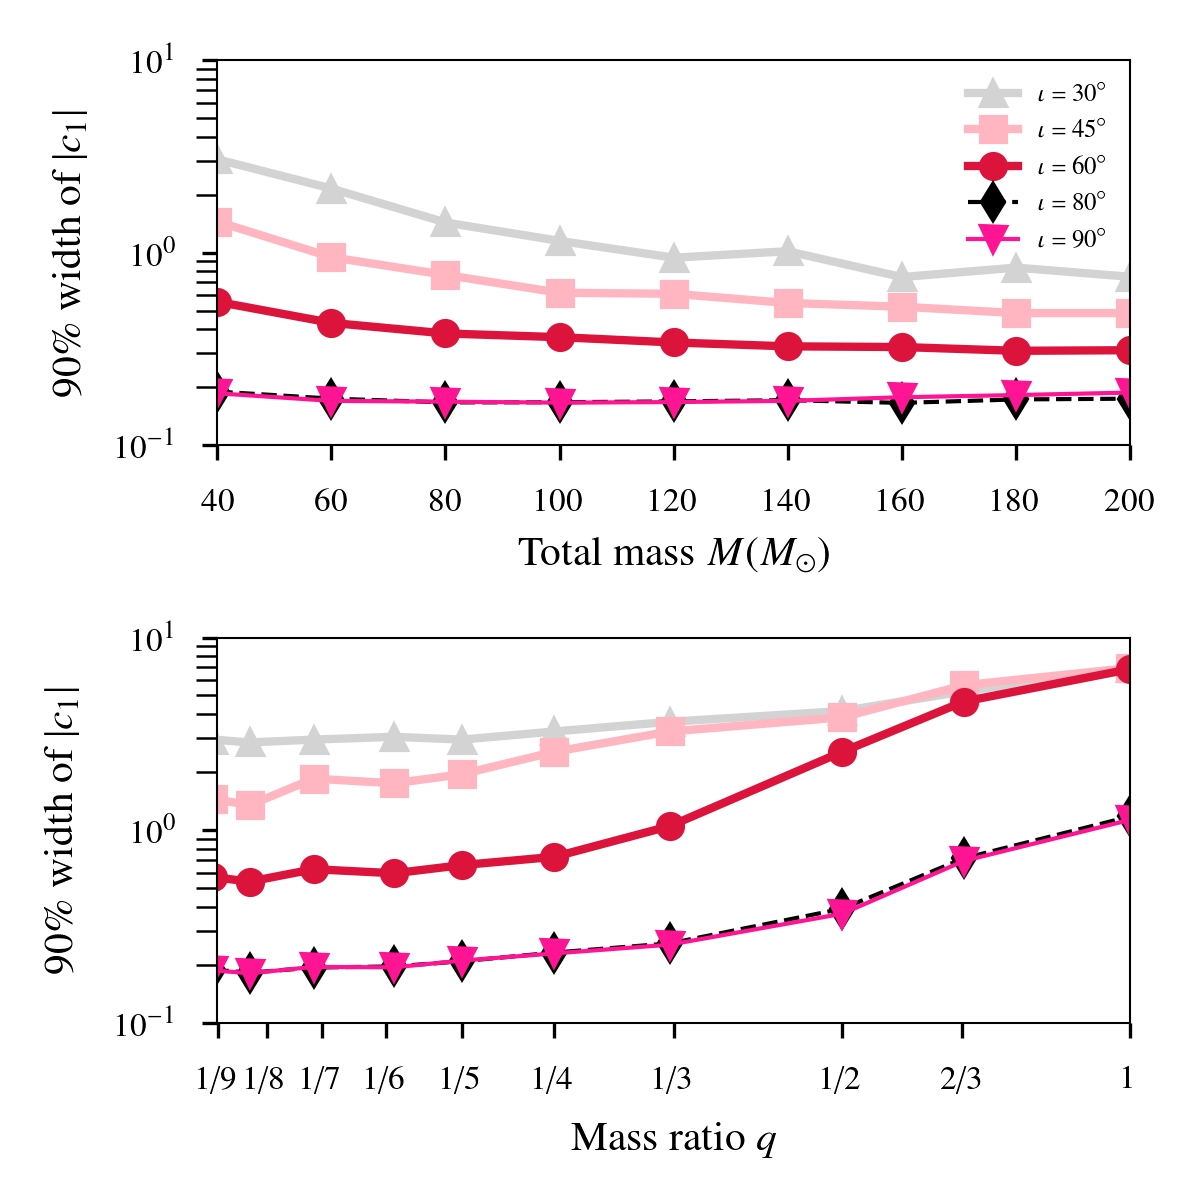
\includegraphics[scale=0.78]{figs/90_percent_CI_c1.png}
	\end{center} 
	\caption{\textbf{FILLER} : The figure shows the width of 90\% credible intervals of $c_1$ for binaries with different total mass $M$ (upper panel)and mass ratio $q$ (lower panel) and inclination angle $\iota$ (legends). All binaries considered in the upper panel have a mass ratio $q=1/9$. Binaries considered in the lower panel have total mass of $40M_{\odot}$. The SNR is set to be 25.  }
	\label{fig:constraint_c1}
\end{figure}
%%%%%%%%%%%%%%%%%%%%%%%%%%%%%%%%%%%%%%%%%%%%%%%%%%%%%

%%%%%%%%%%%%%%%%%%%%%%%%%%%%%%%%%%%%%%%%%%%%%%%%%%%%%
\begin{figure*}[htb]
	\centering
	\subfigure[]{\label{fig:c2_c34}
		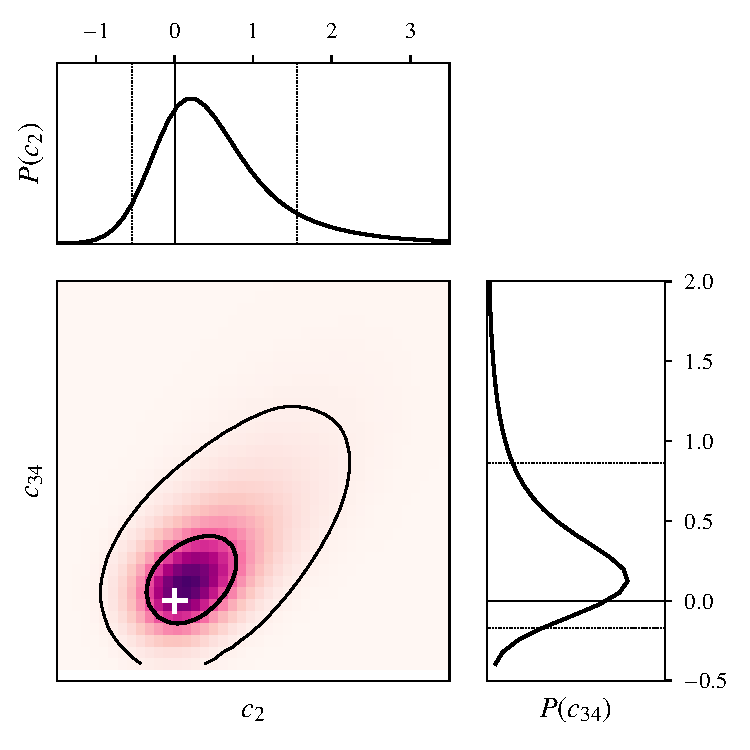
\includegraphics[scale=0.55]{figs/c2_c34_M_80_q_9_SNR_25.pdf}}
	\subfigure[]{\label{fig:c3_c4}
		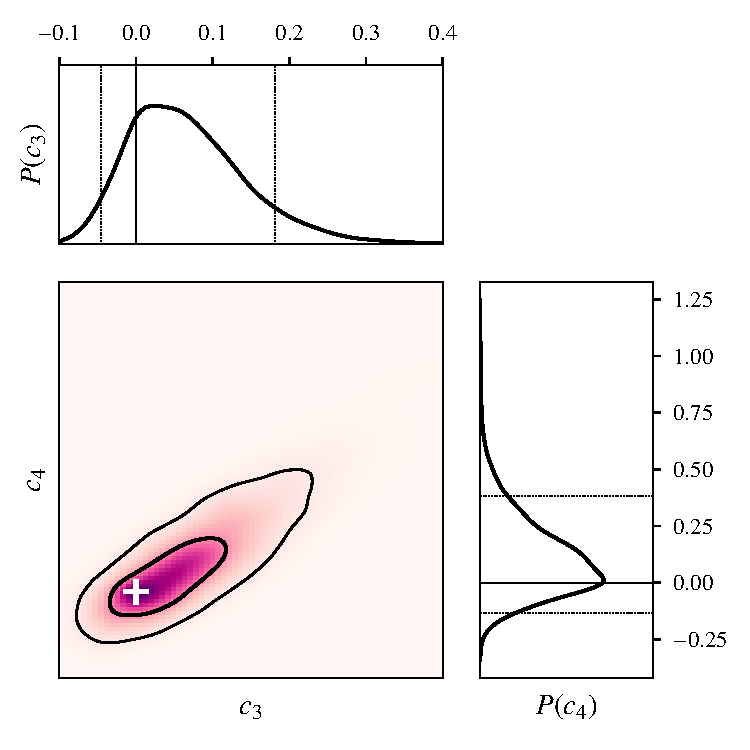
\includegraphics[scale=0.55]{figs/c3_c4_M_80_q_9_SNR_25.pdf}}\\
	\subfigure[]{\label{fig:bounds_c2}
		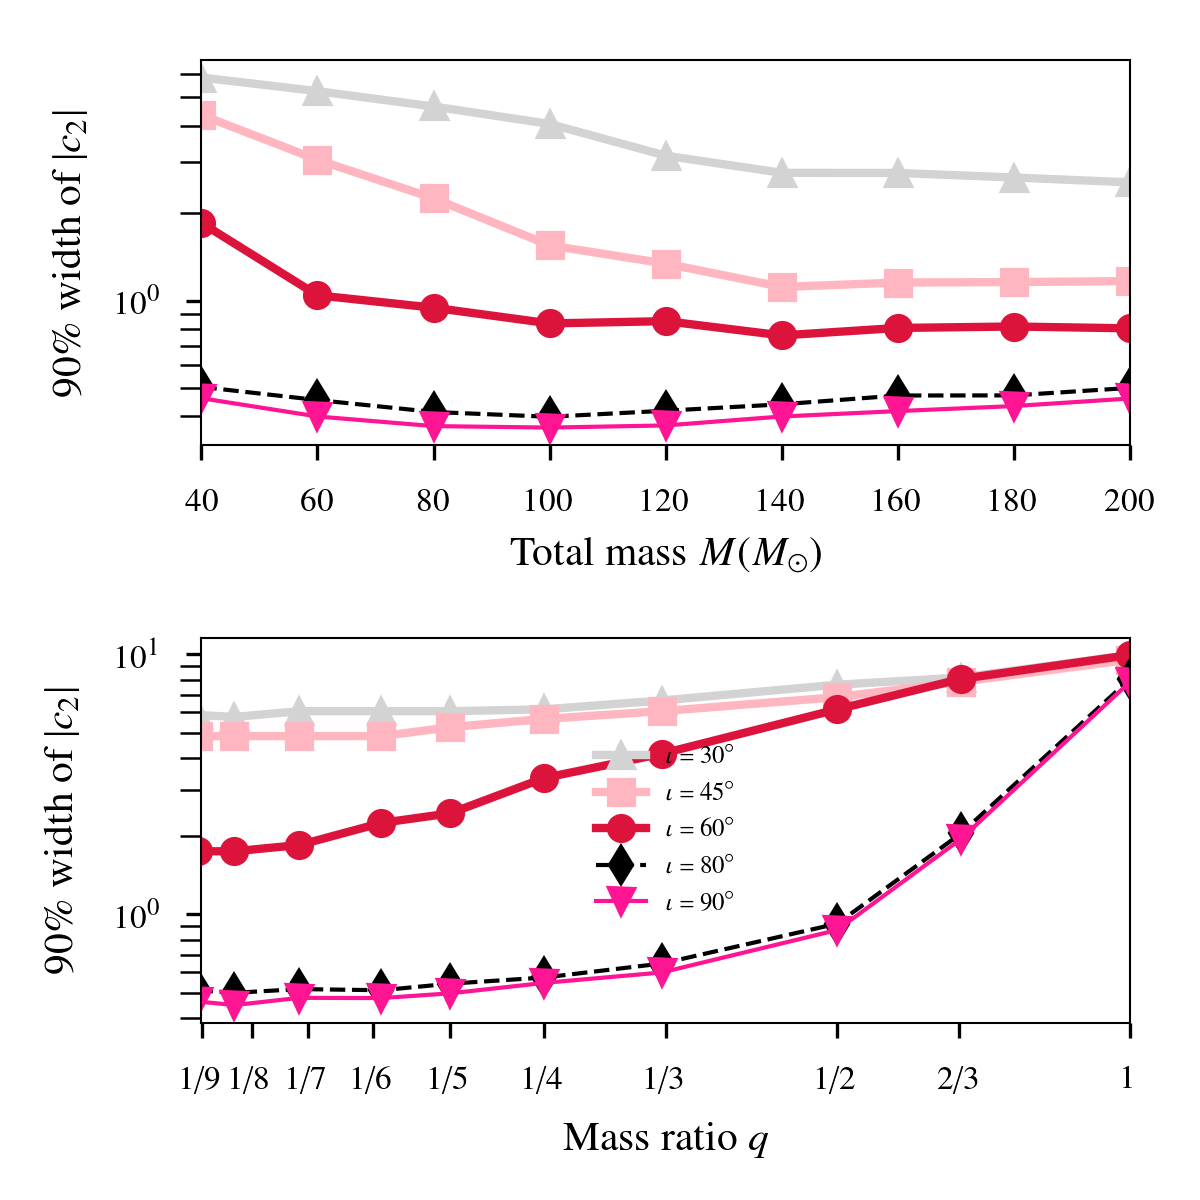
\includegraphics[scale=0.75]{figs/90_percent_bounds_c2.png}}
	\subfigure[]{\label{fig:bounds_c34}
		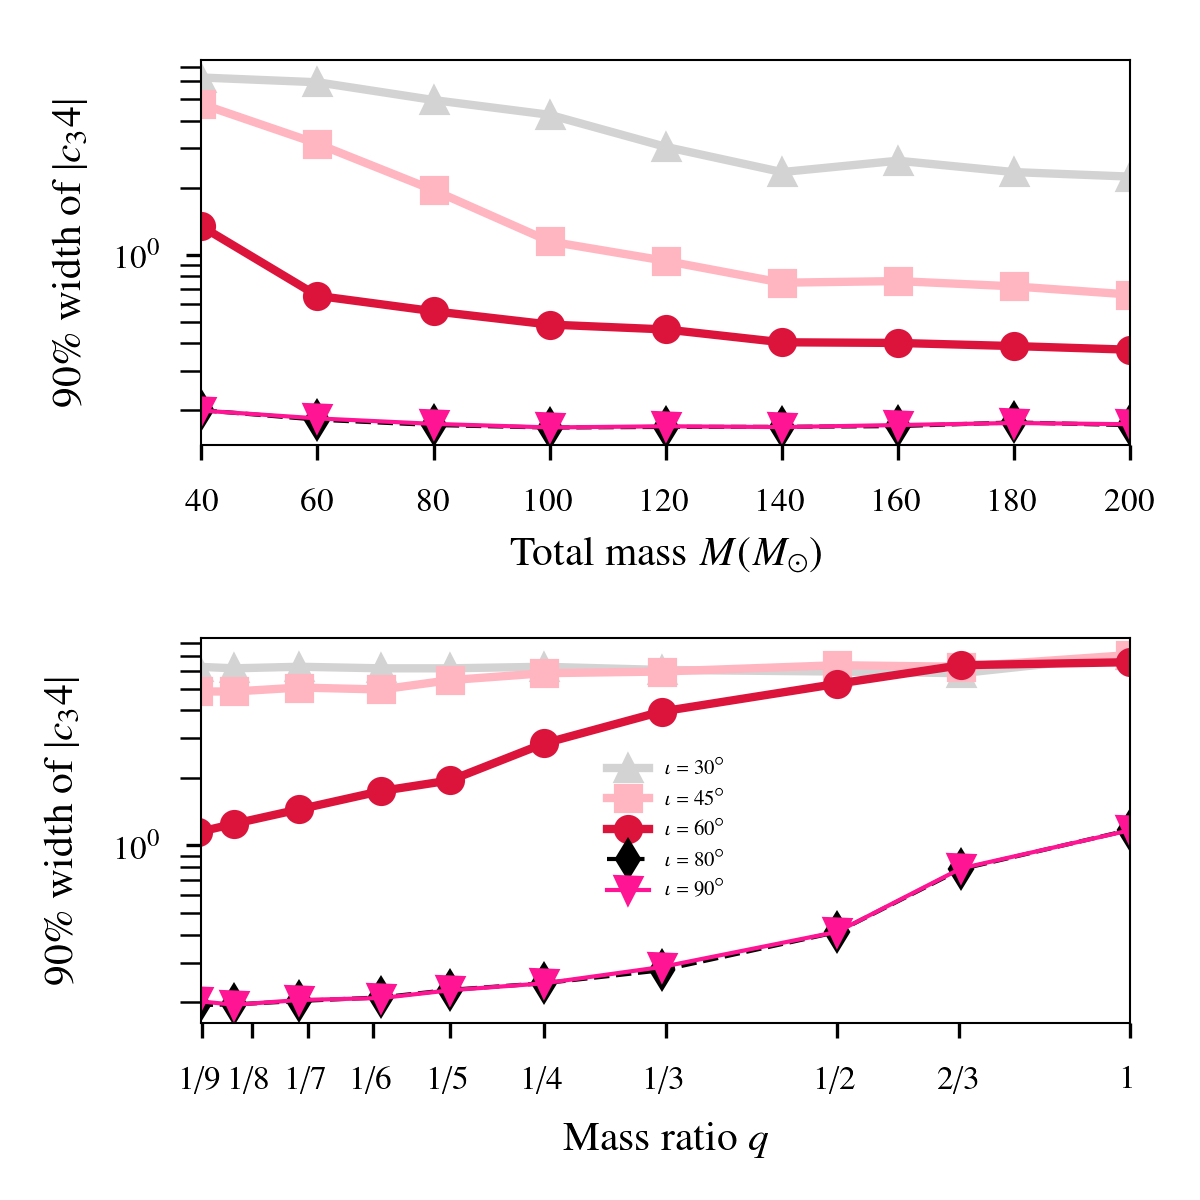
\includegraphics[scale=0.75]{figs/90_percent_bounds_c34.png}}\\
\subfigure[]{\label{fig:bounds_c3}
	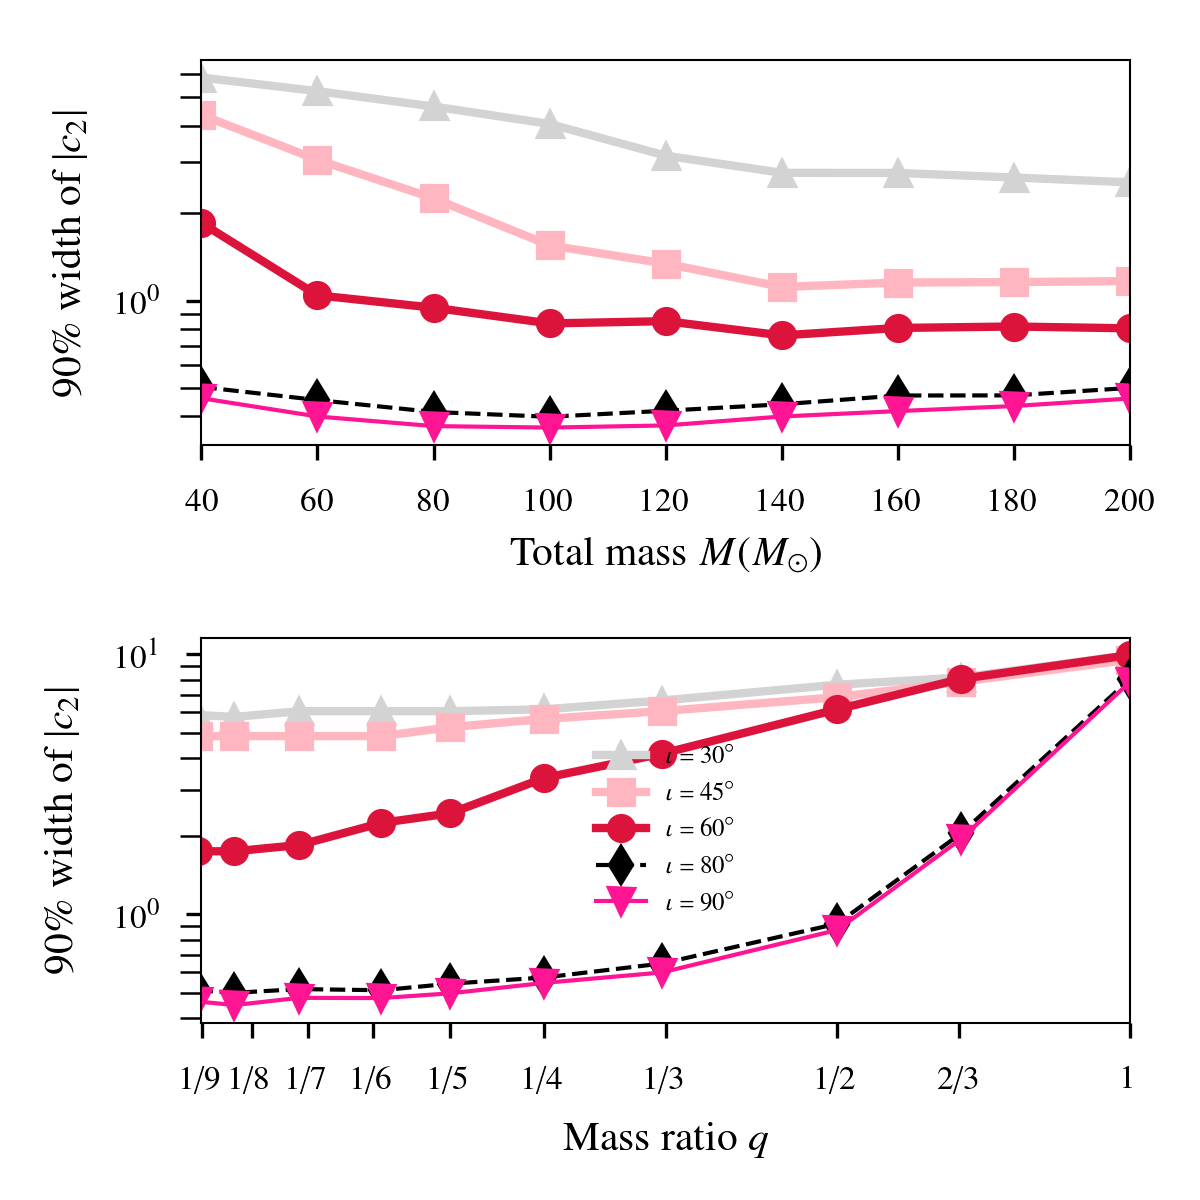
\includegraphics[scale=0.75]{figs/90_percent_bounds_c2.png}}
\subfigure[]{\label{fig:bounds_c4}
	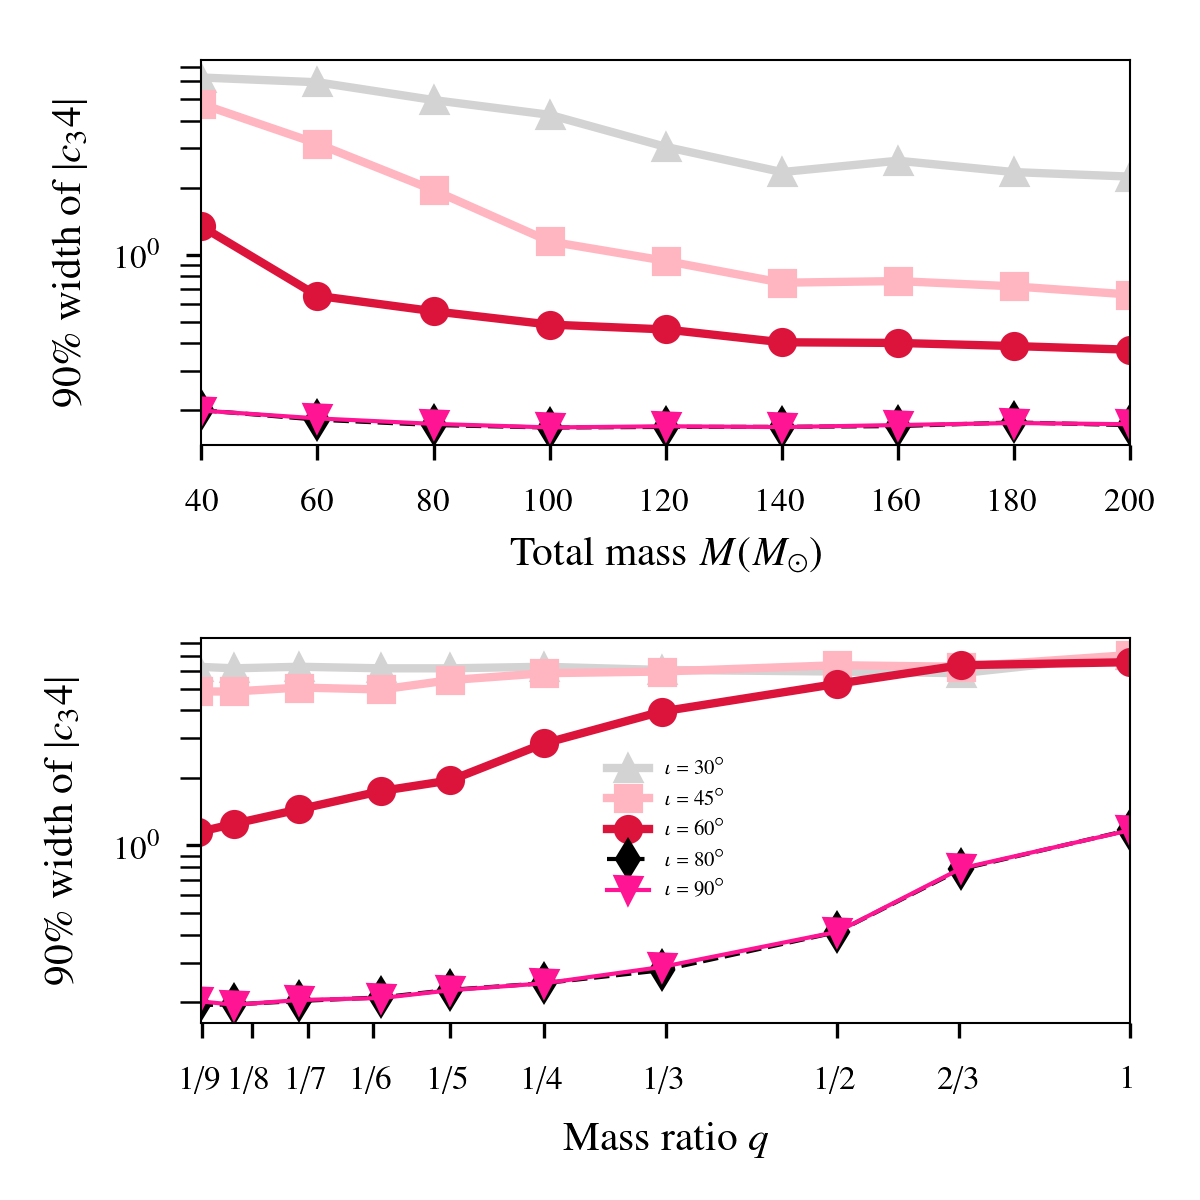
\includegraphics[scale=0.75]{figs/90_percent_bounds_c34.png}}
	\caption{\label{fig:bounds_c2c34c3c4} \textbf{FILLER} : The figure shows the posterior probability distribution of the deviation parameter $c_1$ estimated from the same simulated GR observation in \ref{fig:posterior_BBH_GR_inj}. Same as Fig. \ref{fig:constraint_c1} except the figures reports constraints on the following deviation parameters:
			 (a) $c_2$, (b) $c_{34}$, (c) $c_3$ \& (d) $c_4$. }
\end{figure*}
%%%%%%%%%%%%%%%%%%%%%%%%%%%%%%%%%%%%%%%%%%%%%%%%%%%%%

We observe that the constraints on the deviation parameters become narrower for binaries with large mass ratios ($q < 1/ 2$) and inclination angles ($\iota > 60 ^\circ $). We find that $c_1$ is better constrained than $\{c_3, c_{4}\}$ and $\{c_3, c_{4}\}$. However, the statistical uncertainties in $\Delta \btheta=\{c_1\}$, $\{c_3, c_{4}\}$ and $\{c_3, c_{4}\}$  are modest, reaching only $\sim$ $10^{-1}$. However, this constraints could be significantly improved with third-generation ground/space based detectors. We note that the efficiency of these tests largely depends on the signal-to-noise distribution in the higher modes. The low SNR in the higher modes has resulted prior railing for some of the sample chains of $\{c_3, c_{4}\}$ and $\{c_3, c_{4}\}$ during MCMC sampling for simulated GR events with binaries having smaller values of total mass, mass ratio and inclination angle. Such problems would not arise if the SNR in each of the higher order modes are reasonable high ($\sim 5$). Furthermore, the extrinsic deviation parameter introduced in our tests $\Delta \btheta$ is slightly degenerate with the luminosity distance $d_L$. This degeneracy introduces some uncertainties in our estimation of bounds. 

 %%%%%%%%%%%%%%%%%%%%%%%%%%%%%%%%%%%%%%%%%%%%%%%%%%%%
 \begin{figure}[tbh]
 	\begin{center}
 		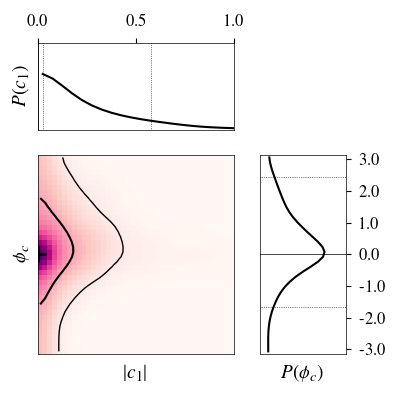
\includegraphics[scale=0.8]{figs/M_80_q_9_SNR_25_complex_c1.png}
 	\end{center} 
 	\caption{The figure shows the posterior probability distribution of the absolute value $|c_1|$and argument $\phi_c$ complex deviation parameter $\tilde{c_1}$ estimated from the simulated GR event. Details are same as in \ref{fig:posterior_BBH_GR_inj}.}
 	\label{fig:c1_complex}
 \end{figure}
 %%%%%%%%%%%%%%%%%%%%%%%%%%%%%%%%%%%%%%%%%%%%%%%%%%%%%
 
A more generalized version of these tests with amplitude correction in the higher modes would be to assume that the deviation parameters $\Delta \btheta$ are complex in nature i.e. they have an amplitude as well as a phase component. To demonstrate such test, we replace the real amplitude correction $c_1$ in Eq. \ref{eq:test_c1} with a complex correction $\tilde{c_1}=|c_1|e^{\phi_c}$. In Fig. \ref{fig:c1_complex}, we show the posterior probability distribution of both the amplitude and phase of the deviation parameter $\tilde{c_1}$. We also estimate the expected bounds on $\tilde{c_1}$ from simulated GR events. We find that though the absolute value of complex correction is well constrained, the phase remains uninformative. 




%%%%%%%%%%%%%%%%%%%%%%%%%%%%%%%%%%%%%%%%%%%%%%%%%%%%%%%%%%%%%%%%%%%%%%%%%%%%%%%%%%%%%%%%%%%%%%%%%%%%%%%%%%%%%%%%%%%%%%%%%%%%%%%%%%%%%%%%%%%%%%%`
\section{Consistency between polarizations}
\label{sec4}
While one can exploit the multipolar structure of the gravitational wave radiation from BBH to formulate efficient tests of GR by introducing intrinsic and extrinsic deviation parameters in the higher order modes, similar tests could be devised with the `two' polarization states of the waveform. We present two such tests in this section and discuss the feasibility of performing such tests with current and future GW observations.
 
\subsection{Consistency between parameters estimated from different polarizations}
The essence of the first test we propose is similar to the test presented in Section \ref{sec3a}. The idea is to estimate the intrinsic parameters $\blambda$ purely from the `plus' polarization of the observed gravitational waveform and then compare it with the estimates obtained from the `cross' polarization of the waveform. In GR, these two independent estimates of $\blambda$ would match. Equivalently, one can introduce deviation parameters $\Delta \blambda := \{\Delta M_c, \Delta q\}$ in the set of intrinsic parameters for $h_\times$ and rewrite the complex time series of gravitational wave radiation as:
\begin{eqnarray} 
\h(t; \blambda, \Delta \blambda) =  h_+(t; \blambda) - ih_\times(t; \blambda, \Delta \blambda),
\label{eq:test_hp_hc}
\end{eqnarray}
and allow a possibility of inconsistency between the `plus' and `cross' polarization states of the signal. We estimate these parameters $\Delta \blambda$ in addition to the standard set of parameters in GR. In GR, we would have $\Delta \blambda = \{0,0\}$. However, if the signal is of non-GR nature, $\Delta \blambda$ would not be consistent with zero.

 %%%%%%%%%%%%%%%%%%%%%%%%%%%%%%%%%%%%%%%%%%%%%%%%%%%%
 \begin{figure}[tbh]
 	\begin{center}
 		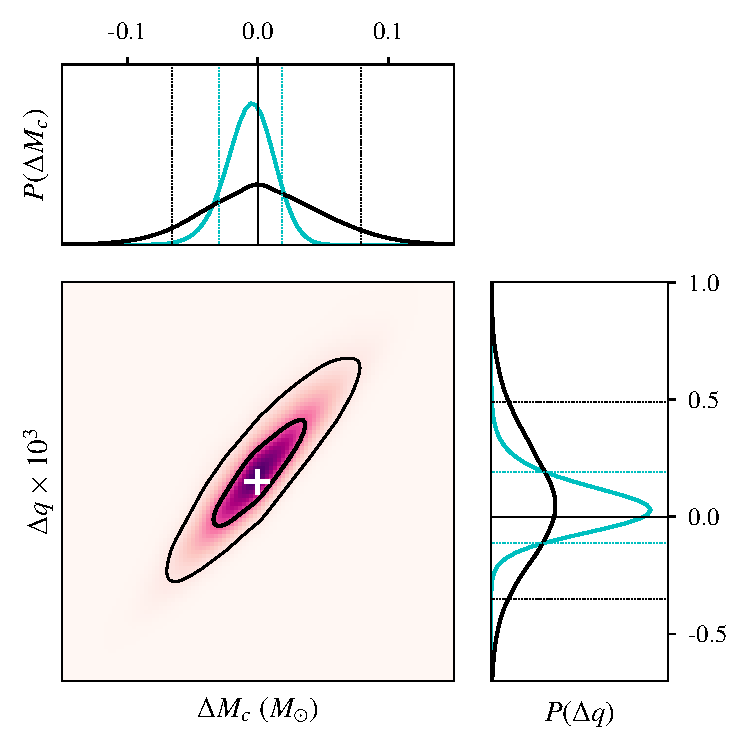
\includegraphics[scale=0.7]{figs/hp_hc_M_80_q_9_SNR_25.pdf}
 	\end{center} 
 	\caption{ Same as \ref{fig:posterior_BBH_GR_inj} but shows the posterior density distributions of $\Delta \blambda$ estimated from the `cross' polarization state.}
 	\label{fig:hp_hc_GR}
 \end{figure}
 %%%%%%%%%%%%%%%%%%%%%%%%%%%%%%%%%%%%%%%%%%%%%%%%%%%%%

In Fig. \ref{fig:hp_hc_GR}, we present the result of the test performed with simulated GR waveform, for a binary with total mass $M = 80M_{\odot}$, mass ratio $q=1/9$, inclination angle $ {\iota}=60^{\circ} $ with a SNR of 25. We first introduce one deviation parameter $\Delta\blambda = {\Delta M_c}$ or $\Delta\blambda = {\Delta q}$ at a time and then perform the test with both the deviation parameters. As expected, the test with only one deviation parameter results a smaller width of the posterior distribution of $\blambda$. Our subsequent analysis of the evolution of the 90\% bounds on $\blambda$ as a function of total mass, mass ratio and inclination angle of the BBH would thus only involve introducing one deviation parameter at a time. In all cases, we set the SNR at 25. In Fig. \ref{fig:hp_hc_90_CI_diffM} and \ref{fig:hp_hc_90_CI_diffq}, we present the expected constraints on ${\Delta M_c}$ and ${\Delta q}$ from simulated GR events. The uncertainties in the deviation parameters reaches well below $10^{-2}$ for both the deviation parameters. Our result shows that this test would prove to be highly efficient in picking up any departure from GR for binaries with large mass ratios ($q < 1/ 2$). Furthermore, it is evident that binaries with smaller inclination angle (even $\iota=30^0$) would also allow a precision test. This particular test thus turns out to be more stringent than the analogous test with higher modes outlined in \ref{sec3a}.  
  
%%%%%%%%%%%%%%%%%%%%%%%%%%%%%%%%%%%%%%%%%%%%%%%%%%%%%
\begin{figure}[h]
	\begin{center}
		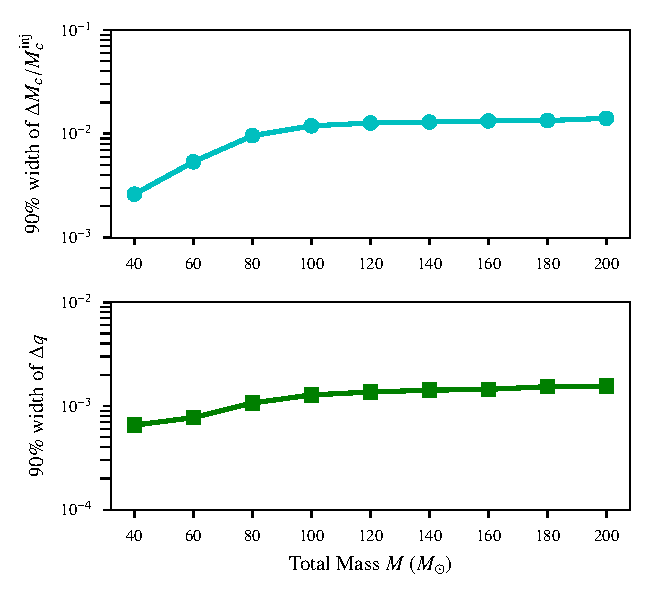
\includegraphics[scale=0.78]{figs/hp_hc_consistency_confidence_interval_varying_M.pdf}
	\end{center} 
	\caption{The figure shows the width of the 90$\%$ confidence limit of the deviation parameters $\Delta M_c$ and $\Delta q$ estimated from the `cross' polarization for binaries with different total mass (horizontal axis) and inclination angles $\iota$ (legends). All binaries have an asymmetric mass ratio $q=1/9$.}
	\label{fig:hp_hc_90_CI_diffM}
\end{figure}
%%%%%%%%%%%%%%%%%%%%%%%%%%%%%%%%%%%%%%%%%%%%%%%%%%%%%

%%%%%%%%%%%%%%%%%%%%%%%%%%%%%%%%%%%%%%%%%%%%%%%%%%%%%
\begin{figure}[h]
	\begin{center}
		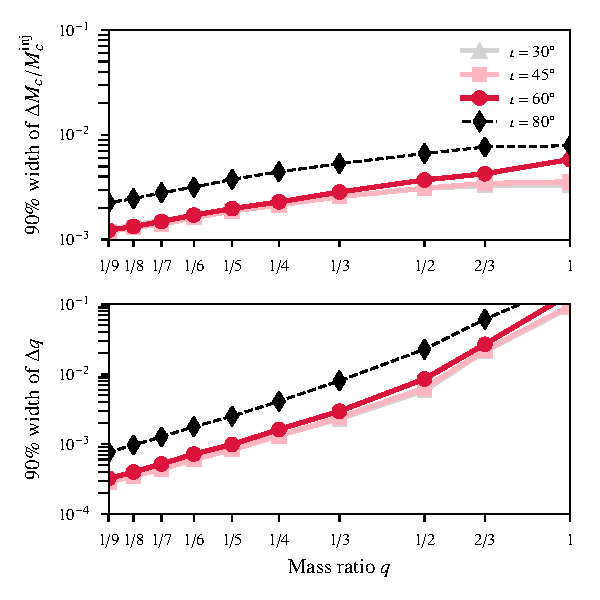
\includegraphics[scale=0.78]{figs/hp_hc_consistency_confidence_interval_varying_q.pdf}
	\end{center} 
	\caption{Same as Fig.~\ref{fig:hp_hc_90_CI_diffM}, except that the horizontal axis reports the mass ratio $q$. All binaries correspond to a total mass $40M_{\odot}$. }
	\label{fig:hp_hc_90_CI_diffq}
\end{figure}
%%%%%%%%%%%%%%%%%%%%%%%%%%%%%%%%%%%%%%%%%%%%%%%%%%%%%

%%%%%%%%%%%%%%%%%%%%%%%%%%%%%%%%%%%%%%%%%%%%%%%%%%%%%%%%%%%%%%%%%%%%%%%%%%%%%%
\subsection{Consistency between the amplitude of different polarizations}
Due to amplitude birefringence, the right (left) circularly polarized gravitational waves are enhanced/suppressed (suppressed/enhanced) compared to the GR expectation as they propagate through cosmological distances. Such birefringence manifests itself through modifying  the `plus' and `cross' polarization. Each of the new `plus' and `cross' polarization is a function of both the `old' `plus' and `cross' polarization in GR and a frequency dependent coupling parameter $v(f)$. Here, we formulate a Chern-Simons gravity (CS) inspired generalized test of \textit{amplitude birefringence}. We introduce an extrinsic deviation parameter (which acts as a coupling parameter in birefringence) $\Delta \btheta=v(f)$. We choose $v(f)$ to be proportional to gravitaional wave frequency $f$ i.e. $v(f)=vf$ with $v$ being a constant. Though this choice of $v(f)$ is motivated by CS gravity, other theories of gravity would also result a frequency dependent modification, maybe with a different exponent for $f$.  The simplistic choice of frequency dependent modification would thus be to assume a liner dependence with $f$.  Our test formalism thus becomes:
 
\begin{eqnarray} 
\h(f; \blambda) =  \Hat{h_+}(f; \blambda) - i \Hat{h_\times}(f; \blambda),
\label{eq:test_cs}
\end{eqnarray}
where $\Hat{h_+}(f; \blambda)=h^{GR}_+ + i v f h^{GR}_{\times}$ and $\Hat{h_\times}(f; \blambda)=h^{GR}_\times - i v f h^{GR}_{+}$. The deviation parameter is exactly zero in GR resulting no \textit{birefringence} at all. However, if the observed signal does not follow GR and show a \textit{birefringence} phenomenon, $v$ would not be consistent with zero any more. In Fig. \ref{fig:cs_hist}, we show an example of the posterior probability density estimated from a simulated GR waveform detected by the Advanced LIGO-VIRGO network for a binary with total mass $M = 80M_{\odot}$, mass ratio $q=1/9$, inclination angle $ {\iota}=60^{\circ} $ with a SNR of 25. 

%%%%%%%%%%%%%%%%%%%%%%%%%%%%%%%%%%%%%%%%%%%%%%%%%%%%%
\begin{figure}[htb]
	\begin{center}
		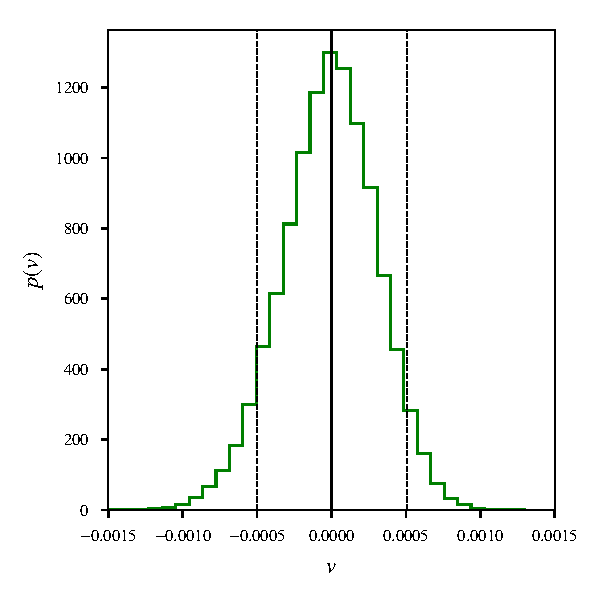
\includegraphics[scale=0.55]{figs/v1_GR_hist_M_80_q_9_dL_250.pdf} 
	\end{center} 
	\caption{Posterior probability density of the deviation parameter $v$ estimated from simulated GR signal for binaries with $M=80$ $M_{\odot}$ and $q=1/9$. }
	\label{fig:cs_hist}
\end{figure}
%%%%%%%%%%%%%%%%%%%%%%%%%%%%%%%%%%%%%%%%%%%%%%%%%%%%%

We then place bounds on $v$ derived from the GR waveforms. We injected waveforms generated from BBH with varying total mass, mass ratio and inclination angle. The width of the computed 90\% credible region for $v$ is shown in Fig. \ref{fig:cs_bounds}. We find that precision tests are possible for wide range of binaries for almost all values of total mass $M$, mass ratio $q$ and inclination angle $\iota$. This corroborates our earlier result that consistency between different states of polarization gives a better test than consistency between different modes. 

%%%%%%%%%%%%%%%%%%%%%%%%%%%%%%%%%%%%%%%%%%%%%%%%%%%%%
\begin{figure}[htb]
	\begin{center}
		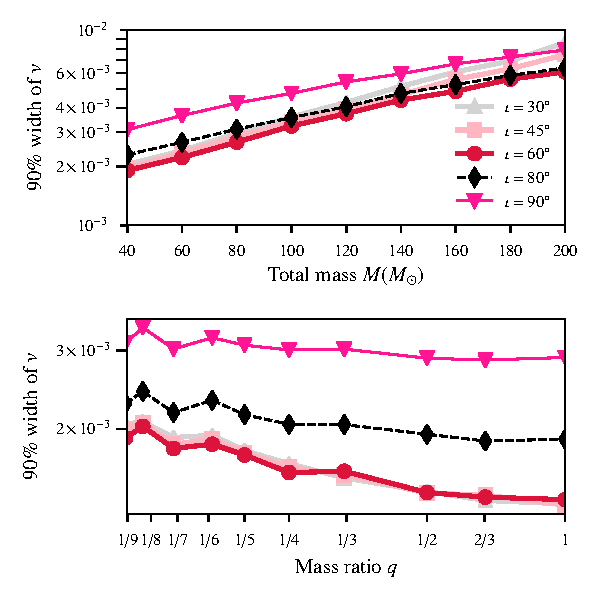
\includegraphics[scale=0.8]{figs/v1_confidence_interval_pol.pdf} 
	\end{center} 
	\caption{The plots shows the width of the 90\% credible region of the deviation parameter $v_1$ estimated from different polarizations of simulated GR signals for binaries with different total mass $M$ and mass ratio $q$. All binaries correspond to a SNR 25.}
	\label{fig:cs_bounds}
\end{figure}
%%%%%%%%%%%%%%%%%%%%%%%%%%%%%%%%%%%%%%%%%%%%%%%%%%%%%

If the GW signal is sufficiently different from that of BBHs in GR and is affected by \textit{amplitude birefringence}, then this test should be able to identity the difference. We demonstrate this by performing the test on a simulated modGR GW signal from a BBH with a total mass of $M = 80 M_\odot$, $q=1/9$ and SNR 60. Figure~\ref{fig:cs_modgr} shows the posteriors of the deviation parameters $v$ estimated from a simulated observation containing this signal, which is \emph{inconsistent} with the GR prediction of $v=0$. The modGR waveform is simulated by incorporating a phenomenological modification to the GR waveform as prescribed in Chern-Simons theory of gravity.

%%%%%%%%%%%%%%%%%%%%%%%%%%%%%%%%%%%%%%%%%%%%%%%%%%%%%
\begin{figure}[h]
	\begin{center}
		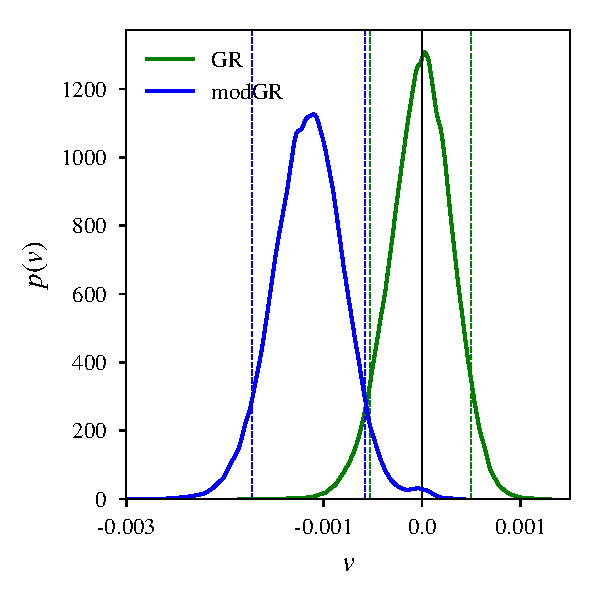
\includegraphics[scale=0.55]{figs/v1_modgr_hist_M_80_q_9_dL_250.pdf} 
	\end{center} 
	\caption{Posterior probability density of the deviation parameter $v$ estimated from simulated GR as well as modGR signal for binaries with $M=80$ $M_{\odot}$ and $q=1/9$. }
	\label{fig:cs_modgr}
\end{figure}
%%%%%%%%%%%%%%%%%%%%%%%%%%%%%%%%%%%%%%%%%%%%%%%%%%%%%

\section{Discussions \& Conclusion}
In this paper, we have proposed a set of four tests of GR using the multipolar structure and different polarization states of the gravitational radiation from a BBH. These tests are, in design, analogous to the `no-hair' tests of BBH with different quasi-normal modes of radiation. We introduced several parameterized deviation parameters in the set of intrinsic and extrinsic sets of parameters in GR and place a constraint on them using a Bayesian framework with simulated GR events.

We first revisited the test of GR, originally presented in~\cite{dhanpal2018}, based on the consistency between the estimates of Chirp mass and mass ratio of the BBH obtained independently from the leading quadrapole mode and the higher order modes; and generalized the test for a network of three realistic Advanced LIGO-VIRGO detectors. The main idea of the test is inspired by the fact that different modes of radiation from the BBH should be uniquely described only by the same values of intrinsic parameters (chirp mass and mass ratio) . Our work illustrates that this formalism would enable one to perform a precision test of GR. However, this test requires appreciable SNR in the higher order modes of the observed GW signal. This severely restricts the number of events for which this test could be performed ($\sim$a few percent); but given LIGO-VIRGO would observed hundreds of BBH mergers in coming years, we expect a reasonable number of such events to be observed.

Furthermore, we check for the consistency between the amplitudes of different modes. In order to do so, we introduce a set of extra deviation parameters in the amplitudes for the higher modes. We consider the deviation parameters to be both real and complex. We find that assuming the deviation to be complex in nature does not give us any additional information. Though this test gives a modest precision with Advanced LIGO-VIRGO detectors, the efficiency of such test is expected to increase manifold with the next generation of detectors (e.g. with Einstein Telescope or LISA). 

We then proceed to formulate two consistency tests of GR using the two different polarization state of the observed signal. We note that, due to \textit{amplitude birefringence}, emitted gravitational waves are affected by a \textit{dephasing} as they propagate through distances. This leads to a `coupling' between `cross' and `plus' polarizations and results a relative enhancement/suppression of the `plus' and `cross' polarization states of the signal, compared to GR,  respectively. We propose two generic tests which can identify any such inconsistency with GR. Our first test  looks for any inconsistency in the estimates of the intrinsic parameters inferred from the two polarizations of the observed signal independently. In the second case, we conceptualize an extrinsic deviation parameter describing the strength of `coupling' (which is a measure of departure from GR; in GR, the deviation parameter would be zero) in the waveform and constrain it with simulated GR events. We demonstrate that both these tests would be highly efficient to detect any non-GR characteristic in the observed GW signal. 

All bounds on the generalized deviation parameters reported in this paper have been obtained by performing the respective tests with only one simulated events. The constraints could be improved by performing the tests with combined set of simulated events.  
\newpage
\bibliographystyle{apsrev-nourl}
\bibliography{TestGR.bib}

\end{document}
